\chapter{Analyse et spécification des besoins}
\label{chap:besoins}

% \section{Acteurs du système}

% Le tableau~\ref{tab:acteurs} décrit les acteurs. Sur le plan métier, une personne physique
% est modélisée par un \texttt{User} rattaché à un tenant ; elle joue un ou plusieurs rôles
% via l'entité \texttt{Actor} (consommateur et/ou fournisseur). Le contrôle d'accès
% applicatif repose sur un ensemble de rôles (\texttt{USER}, \texttt{ADMIN},
% \texttt{PROVIDER}, \texttt{CONSUMER}).

% \begin{table}[H]
% \centering
% \caption{Acteurs du système}
% \label{tab:acteurs}
% \renewcommand{\arraystretch}{1.3}
% \begin{tabularx}{\linewidth}{L{3cm} X L{3.2cm}}
% \toprule
% \textbf{Acteur} & \textbf{Description} & \textbf{Rôles possibles} \\
% \midrule
% Tenant     & Organisation cliente ; contexte d'isolation des données et configurations & --- \\
% User       & Identité authentifiable rattachée à un tenant & USER, ADMIN, PROVIDER, CONSUMER \\
% Consumer (CdS) & Acteur demandeur de services & CONSUMER \\
% Provider (FdS) & Acteur fournisseur de services & PROVIDER \\
% Admin      & Administrateur (plan de contrôle) & ADMIN \\
% \bottomrule
% \end{tabularx}
% \end{table} 
\section{Besoins fonctionnels}

Les besoins fonctionnels sont identifiés par un code \texttt{F-XXX-NNN}. Les
tableaux~\ref{tab:bf-identite} à~\ref{tab:bf-facturation} les regroupent par domaine.

\begin{table}[H]
\centering
\caption{Besoins fonctionnels --- Identités (Tenant, User, Actor)}
\label{tab:bf-identite}
\renewcommand{\arraystretch}{1.25}\footnotesize
\begin{tabularx}{\linewidth}{L{2cm} L{4.6cm} X}
\toprule
\textbf{ID} & \textbf{Fonctionnalité} & \textbf{Contraintes} \\
\midrule
F-TEN-001 & Provisionner un tenant (inscription publique) & Nom et domaine obligatoires, \texttt{tenant\_id} UUID généré \\
F-USR-001 & Inscrire un utilisateur (register) & Email unique, mot de passe chiffré (BCrypt) \\
F-USR-002 & Authentifier (login) & Retourne un JWT portant rôles et \texttt{tenantId} \\
F-USR-003 & Gérer les rôles d'un utilisateur & Réservé au rôle ADMIN \\
F-ACT-001 & Créer un acteur lié à un utilisateur & Un utilisateur peut avoir plusieurs acteurs \\
F-ACT-002 & Filtrer les acteurs par rôle & --- \\
\bottomrule
\end{tabularx}
\end{table}

\begin{table}[H]
\centering
\caption{Besoins fonctionnels --- Métiers (Business, Rule, Catalogue, Resource, Media, Portfolio)}
\label{tab:bf-metier}
\renewcommand{\arraystretch}{1.25}\footnotesize
\begin{tabularx}{\linewidth}{L{2cm} L{4.6cm} X}
\toprule
\textbf{ID} & \textbf{Fonctionnalité} & \textbf{Contraintes} \\
\midrule
F-BUS-001 & Créer / modifier un métier & Nom et domaine obligatoires ; rattaché au tenant \\
F-BUS-002 & Rechercher par domaine & --- \\
F-BRU-001 & Définir une règle métier (clé--valeur) & Rattachée à un Business \\
F-SCA-001 & Créer un service au catalogue & Prix de base + devise validée \\
F-SCA-002 & Filtrer les services disponibles & \texttt{isAvailable} \\
F-RES-001 & Gérer une ressource (stock) & Quantité $\geq 0$ \\
F-MED-001 & Associer un média à un métier & Type + URL \\
F-POR-001 & Gérer un portfolio de compétences & 1 portfolio par acteur ; relation N:M avec Business \\
\bottomrule
\end{tabularx}
\end{table}

\begin{table}[H]
\centering
\caption{Besoins fonctionnels --- Transactions (ServiceRequest, Invoice, Message, Notification)}
\label{tab:bf-facturation}
\renewcommand{\arraystretch}{1.25}\footnotesize
\begin{tabularx}{\linewidth}{L{2cm} L{4.6cm} X}
\toprule
\textbf{ID} & \textbf{Fonctionnalité} & \textbf{Contraintes} \\
\midrule
F-SRE-001 & Créer une demande de service (CdS) & Consumer, provider et service du catalogue requis \\
F-SRE-002 & Faire évoluer le statut & FSM : accept / start / fulfill / cancel \\
F-SRE-003 & Suivre par statut / acteur & --- \\
F-INV-001 & Générer une facture & Automatique à la finalisation (ACK) \\
F-INV-002 & Payer / annuler une facture & FSM : pay / cancel \\
F-MSG-001 & Échanger des messages sur une demande & Temps réel (publication/abonnement) \\
F-NOT-001 & Notifier un utilisateur & Compteur de non-lus, marquage lu \\
F-AUD-001 & Tracer les événements (audit) & Par \texttt{traceId}, acteur, tenant \\
F-ANA-001 & Calculer les KPIs d'un tenant & --- \\
\bottomrule
\end{tabularx}
\end{table}

\section{Besoins non fonctionnels}

Le sujet impose un ensemble exigeant de contraintes non fonctionnelles. Le
tableau~\ref{tab:bnf} en précise le statut dans le présent MVP, dans une logique de
transparence : ce qui n'est pas pleinement réalisé est repris comme perspective au
chapitre~\ref{chap:perspectives}.

\begin{table}[H]
\centering
\caption{Besoins non fonctionnels et statut dans le MVP}
\label{tab:bnf}
\renewcommand{\arraystretch}{1.3}\footnotesize
\begin{tabularx}{\linewidth}{L{3.2cm} X C{2.4cm}}
\toprule
\textbf{Besoin} & \textbf{Description} & \textbf{Statut MVP} \\
\midrule
Multi-tenant & Isolation des données par tenant sur infrastructure partagée & Réalisé \\
Sécurité & Authentification JWT, mots de passe chiffrés, RBAC & Réalisé \\
Multi-devises & Support XAF, XOF, NGN, KES, GHS, USD, EUR, GBP & Réalisé \\
Documentation API & Spécification OpenAPI / Swagger UI & Réalisé \\
Conteneurisation & Docker / docker-compose & Réalisé \\
Modularité (DDD / hexagonal) & Monolithe modulaire, microservices-ready & Réalisé \\
Temps réel & Messagerie instantanée sur les demandes & Partiel (Redis pub/sub) \\
Événementiel & Bus d'événements (notifications, audit) & Partiel (infra posée) \\
Géo-référencement & PostGIS, géolocalisation native & Perspective \\
Offline-first / PWA & Application installable et hors-ligne & Perspective \\
Internationalisation & i18n web et mobile & Perspective \\
Réactif & WebFlux + R2DBC non bloquant & Perspective \\
2FA & Double authentification & Perspective \\
Mobile natif & React Native & Perspective \\
\bottomrule
\end{tabularx}
\end{table}

\section{Diagramme de contexte}
\begin{figure}[H]
    \centering
    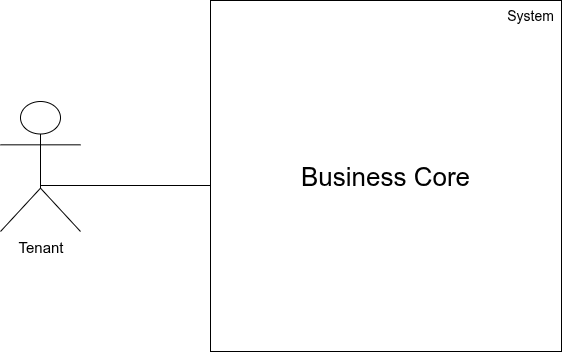
\includegraphics[width=0.8\linewidth]{chapitres/diagramme de contexte.drawio.png }
    \captionof{figure}{Diagramme de contexte du système}
    \label{fig:placeholder}
\end{figure}
